\section{Program til konvertering af billede til G-kode}

\lstset{
 basicstyle=\fontsize{11}{13}\selectfont\ttfamily,
 numbersep=3pt,breaklines=true
}

I dette afsnit vil der først komme en gennemgang af koden, der er skrevet i Mathematica. Efter dette kommer et afsnit med overvejelser og valg i forbindelse med koden. I gennemgangen af koden vil der blive vist nogle brudstykker af koden - den fulde kode kan findes på den vedlagte DVD. Formålet, med den Mathematica kode der laves, er, at man kan konvertere et billede eller logo til G-kode. Koden fungerer ved, at man åbner og evaluerer Mathematica-filen. Herved åbnes et GUI, hvori man kan uploade et billede. I dette GUI kan man indstille forskellige ting, som f.eks. hvor mange pixels, der skal være, og om det er et billede eller logo. Når man er færdig med indstillingerne, trykker man "save G-kode". Herved genereres G-koden ud fra indstillingerne og gemmes som en .nc fil, der kan bruges i simuleringen til robotten.
\subsection{Opbygning af Mathematica kode}
Selve programmet til at konvertere et valgt billede til G-kode, er delt op i tre dele og sat ind i et GUI. De tre dele består af en del til billeder, og to dele til logoer. De tre dele minder meget om hinanden -der er dog forskel på opbygningen af dem, og den måde de agerer på. Delen til billeder kører med tre forskellige gråtoner. De to dele til logoer kører kun med farverne sort og hvid. Den ene tegner kanten rundt om et logo, mens den anden fylder logoet.

Mange af de ting, der indgår i koden, er konceptuelle, og vil derfor ikke blive beskrevet her, mens der vil blive lagt mere vægt på de mere interessante dele af koden. De konceptuelle ting er bl.a. nogle konstanter, der har forskellige værdier - herunder startværdier for forskellige variabler, og konstanter for spidsning og lignende. Billedet, der skal laves til G-kode, bliver i alle tre dele importeret med kommandoen Import. Billedet bliver herefter behandlet forskelligt alt afhængigt af, om det er et logo eller et billede.
\subsubsection{Konvertering af billede til G-kode}
I dette afsnit vil delkoden, der konverterer billedet til G-kode, blive gennemgået.

\textbf{Behandling af billedet}\\
\begin{figure}[h]
	\begin{lstlisting}
bil=ImageData[ColorQuantize[ImageResize[ColorConvert[g,"Grayscale"],a],3,Dithering -> False]]
\end{lstlisting}
	\caption{Behandlingen af billedet}
	\label{fig:bil}
	\end{figure}
Efter billedet er blevet importeret, bliver det behandlet med flere indbyggede funktioner fra Mathematica. Dette kan ses på figur~\ref{fig:bil}. Der bliver brugt en funktion, der hedder ColorConvert. Denne funktion bruges til at lave billedet om, så det kun består af gråtoner. Dernæst bruges en kommando kaldet ImageResize, der gør det muligt, at bestemme hvor mange pixels billedet skal bestå af. Den sidste kommando, der bliver brugt til at behandle billedet, er ColorQuantize. Med denne kommando kan man lave billedet om til at bestå af et færre antal farver. I tilfældet med denne kode er det valgt, at billedet skal bestå af tre farver, og da det i forvejen var lavet til gråtoner, kommer det til at bestå af tre gråtoner.

Efter billedet er blevet behandlet, udtrækkes dataene fra billedet vha. en funktion kaldet ImageData. På denne måde fås en matrix, hvor hvert tal i matrixen beskriver en farve for en pixel, og da der er tre forskellige gråtoner, vil der indgå tre forskellige talværdier i matrixen - en for hver gråtone.

\textbf{"Spidskode" til spidsning af blyant}\\
\begin{figure}[h]
	\begin{lstlisting}
spidskode:="N"<>ToString[n++]<>" G98 Z"<>ToString[nulpunkt+bly]
 \end{lstlisting}
	\caption{G-kode linje for spidsning}
	\label{fig:spidskode}
	\end{figure}
For at styre linjenumrene i G-koden laves en variabel N, der tæller en op, hver gang der laves en G-kode linje. Z-værdien i G-koden er tilpasset således der bliver taget højde for slid og placeringen på tegneplanet. På den måde er der hele tiden er et konstant tryk, så der kan blive tegnet. Ser man på en G-kode linje for en spidsekommando, ses det at denne kun skal have tre argumenter. Denne G-kode linje for spidsning kan ses på figur~\ref{fig:spidskode}. Z-værdien er givet ved sliddet, der ved hver spidsning bliver regnet ud til et nyt nulpunkt. Til dette nulpunkt er der lagt et konstant tryk til, da blyantsspidsen ved Z0 er i plan med blyantspidserens top. Denne G-kode funktion for spidsning af blyantspidseren er ens gennem hele programmet. 

\textbf{Yderste del af G-kode funktionen}\\
\begin{figure}[h]
	\begin{lstlisting}
For[i=1,i<b,i++,
  For[iq=Union[bil[[i]]]; wq=3;, 
   Length[Select[iq,#<bild[[wq]]&]]>0,wq--;,
   gg = den i'te liste med to af de lyseste punkter i hver ende
   If[wq==2,kode;kode,kode]]];
 \end{lstlisting}
	\caption{Yderste del af G-kode funktionen}
	\label{fig:ydregkode1}
	\end{figure}
Kigger man på koden udefra og ind, kan man skabe sig et lidt bedre overblik. Dette kan ses på figur~\ref{fig:ydregkode1}. Det ønskes, at den mest lyse gråtone skal være hvid, og tegnes derfor ikke. Den midterste gråtone skal være grå og dermed kun tegnes en gang, og den tredje og mørkeste gråtone skal tegnes flere gange for at opnå den mørke farve. Da det ønskes at tegne som en printer, tages der udgangspunkt i en linje af gangen. Dette gøres ved at lave en for løkke, der løber fra 1 til antallet af rækker i matrixen med billeddataene. Med dette kan man nu i for løkken fokusere på en række af gangen. I denne for løkke er en anden for løkke, som først tester om den i'te række indeholder nogle gråtoner, der skal tegnes. Derefter tester for løkken om rækken indeholder punkter med den mørkeste gråtone, der så skal tegnes flere gange. Hvis testen er sand, laves der en liste med den i'te række af billeddataene. I hver ende af denne liste bliver der tilføjet to værdier, som svarer til den lyseste gråtone, der altså ikke skal tegnes. Viser det sig, at der er noget i den i'te række, der skal tegnes, når løkken kører første gang, køres funktionen "kode" en gang. Hvis det er anden gang løkken kører, og der er nogle punkter af den mørke gråtone i den i'te række, så køres funktionen kode to gange. Alt dette vil resultere i, at den lyseste gråtone ikke bliver tegnet, den midterste gråtone bliver tegnet en gang, og den mørkeste gråtoner bliver tegnet i alt tre gange.

\textbf{Opbygning af funktionen "kode"}\\
\begin{figure}[h]
	\begin{lstlisting}
kode := If[Er linjen ulige, ww = Append[ww, Table[
       If[Er der et tegnepunkt,
        If[Er alle tre punkter tegnepunkter,
         counter++; If[Skal der spidses,
          {tegnluft1, luft1, spidskode, spidskode, spidskode, luft1, 
           tegnluft1}, Ellers intet],
         If[Skal der spidses, {tegnluft1, luft1, spidskode, spidskode, 
           spidskode, luft1, tegnluft1},
          tegnluft1]], Ellers intet]
       , fra 2 til x dimensionen + 3]];,
   Ellers tegne fra den anden vej];
 \end{lstlisting}
	\caption{Opbygningen af funktionen G-kode}
	\label{fig:opbygninggkode1}
	\end{figure}
Ser man lidt nærmere på funktionen "kode"s opbygning, ses det, at den er opbygget af hovedsageligt if og table kommandoer. Dette kan ses på figur~\ref{fig:opbygninggkode1}. Først tester den om linjen skal tegnes fra den ene eller anden side -dette gøres vha. en OddQ funktion, der tester på en variabel, som tæller en op, hver gang der er tegnet en linje. Hvis OddQ er sandt, bruges der en Append. På den måde bliver der tilføjet en liste fra table til listen ww. Tablen kører hvor den ændrer j fra 2 til længden af rækken og lægger tre til. Inde i tablen testes det først med en if kommando om et eller flere af tre punkter, der kommer efter hinanden, skal tegnes. Hvis dette er tilfældet, testes der igen med en anden if kommando, hvis ikke det er rigtigt, sker der ikke noget. Vha. denne nye if kommando testes det, om alle de tre punkter skal tegnes; skal de det, tælles counter først en op. Counter er en variabel, der tæller en op, hver gang der bliver lavet en tegne G-kode. Efter counter er talt op, testes det om blyanten skal spidses - hvis den skal, laves der et nyt nulpunkt, hvor sliddet er lagt til det tidligere nulpunkt. Counter sættes til 1, og der laves en liste af tegnluft1, luft1, spidsekode, spidsekode, spidsekode, luft1 og tegnluft1. Dette gør, at blyanten først bliver løftet og derefter spidses den tre gange. Herefter kommer den på plads med en luftkode, og fortsætter med at tegne. Begrundelsen for disse valg kommer senere under afsnittet om overvejelser og valg. Hvis testen viser, at blyanten ikke skal spidses, vil counter blive talt en op. Hvis ikke alle de tre punkter, der testes, skal tegnes, testes det alligevel om blyanten skal spidses. Dette gøres på samme måde som tidligere. Hvis den ikke skal spidses, køres funktionen tegnluft1. Går man tilbage til testen af, hvilken retning der skulle tegnes fra, kan man se, at når der tegnes fra den modsatte side en først beskrevet, er der indsat en konstant, og j er trukket fra. På denne måde tæller det ned i stedet for at tælle op.

\textbf{Tegne- og luftfunktioner}\\
\begin{figure}[h]
	\begin{lstlisting}
tegnluft1 := "N" <> ToString[n++] <>
   " G0" <> ToString[If[Er det et luft punkt, 0, 1]] <>
   " X" <> ToString[Pxd*(j - 2) - forskyda] <>
   " Y" <> ToString[Pxd*i - forskydb] <>
   " Z" <> ToString[If[Er det et tegnepunkt, 
     counter++; (nulpunkt + slidprPx*(counter - 1) + konstanttryk + Z[i*Pxd - forskydb]),
     If[Er Z mellem 0.00001 og - 0.00001, 
      substitueres 0.0001 fra luft; (nulpunkt + slidprPx*(counter - 1) +luft),
      (nulpunkt + slidprPx*(counter - 1) + luft)]]];
 \end{lstlisting}
	\caption{Opbygningen af funktionen tegnluft1}
	\label{fig:tegnluft1}
	\end{figure}
Det kan ses, at de fire funktioner luft1, luft2, tegnluft1 og tegnluft2 minder meget om hinanden. Derfor kigges her kun nærmere på funktionen tegnluft1. Tegnluft1 er en funktion, der laver en G-kode linje. Funktionen tegnluft1 kan ses på figur~\ref{fig:tegnluft1}. Linjenummeret bestemmes som tidligere beskrevet. Efter det testes det, om dette er en luft eller tegne G-kode linje, der skal laves, hvilket afgører, om der skrives G00 eller G01. Efter dette bestemmes X- og Y-værdierne ud fra koordinaterne til punktet. Der fratrækkes en forskydningsværdi fra koordinaterne til punktet, for at centrere billedet på midten af papiret, da X0 og Y0 ligger i centrum af papiret. Det sidste, der bliver beregnet i funktionen, er Z-værdien. Denne værdi bestemmes ved først at teste, om det er et tegne- eller luftkoordinat. Er det et tegne koordinat lægges der en til counter, og Z-værdien bestemmes som nulpunktet lagt sammen med sliddet, det konstante tryk og den værdi, der er som følge af placeringen på planet. Hvis det er et luftpunkt, testes der først om værdien vil blive for lille. Er den det trækkes der 0.1mm fra variablen luft. Z-værdien bestemmes så ved at lægge nulpunktet, sliddet og luft sammen. Her gør konstanten, at luftpunktet bliver hævet ca 1cm over planet, så der dermed ikke tegnes.

\textbf{Eksportering af G-kode}\\
Når alt dette er kørt igennem, vil listen ww indeholde al G-koden. Altså er hver punkt på listen en G-kode linje på string form. Denne liste eksporteres som en tekstfil til en valgt placering. Herefter oprettes der en batch fil, der kan lave den bestemte fil om til en .nc fil. Denne batch fil køres, hvorefter den slettes igen. Efter dette er G-koden færdig og skrevet som en .nc fil, der kan køres i simuleringen til robotten.
\subsubsection{Konvertering af logo til G-kode}
Der kigges nu på den del af programmet, der arbejder med et logo i stedet for et billede. Denne logo-del kan opdeles i to dele: En del der udfylder logoet, og en del der laver kanten. Den del, der laver G-koden til fyldet af logoet, minder meget om den del, der laver et billede om til G-kode, da de begge vil tegne på samme måde -forskellen er, at der ved logoet kun tegnes én gråtone. 

\textbf{Behandling af logoet}\\
\begin{figure}[h]
	\begin{lstlisting}
jk = MorphologicalBinarize[ImageResize[g, a], {s1, s2}]
 \end{lstlisting}
	\caption{Behandling af logo}
	\label{fig:jk}
	\end{figure}
Både delen til kanten og til fyldet skiller sig ud fra billeddelen i form af deres behandling af billedet. Efter det er importeret, bruges funktionen ImageRezise for at få billedet med det antal pixel, der ønskes. Herefter bruges der en indbygget funktion (kaldet MorphologicalBinarize) til at behandle billedet. Dette kan ses på figur~\ref{fig:jk}. Funktionen laver billedet om til sort og hvid. Det fungerer ved, at den tager udgangspunkt i en øvre og nedre grænse for kontrasterne, og ud fra disse værdier bestemmes det hvor meget, der skal være sort. Man har via GUIen mulighed for at vælge automatisk - så funktionen selv finder grænserne - man kan vælge selv at bestemme den øvre grænse, eller selv at bestemme både den øvre og nedre grænse.

Da resten af den del, der laver G-koden til fyldet af logoet, minder meget om delen, der laver billedet til G-koden, vil denne del ikke blive beskrevet yderligere. I stedet vil der blive kigget lidt nærmere på den del, der laver G-koden til kanten af logoet.
\begin{figure}[h]
	\begin{center}
	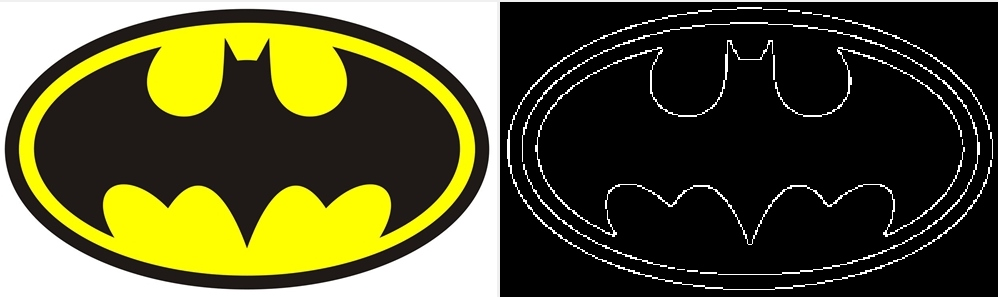
\includegraphics[scale=0.4]{Billeder/edgedetect.jpg}
	\caption{Et eksempel på brugen af EdgeDetect}
	\label{fig:edgedetect}
	\end{center}
\end{figure}
I delen, der laver kanten, bliver logoet yderligere behandlet med en funktion, der hedder EdgeDetect. Denne funktion finder kanten hele vejen rundt om logoet. Et eksempel på dette kan ses på figur~\ref{fig:edgedetect}. Bagefter bruges funktionen ImageData, hvorved man får en matrix, der indeholder alle punkterne, hvor kanten af logoet er givet ved 1-taller, og resten er givet ved nuller.

\begin{figure}[h]
	\begin{lstlisting}
list2=Prepend[Position[bil, 1][[Last[FindShortestTour[
	Position[bil,1]]]]],{-2,-2}];
 \end{lstlisting}
	\caption{Opbygningen af list2}
	\label{fig:list2}
	\end{figure}
For at komme til at tegne kanten af logoet mest effektivt, anvendes funktionen FindShortestTour, hvilket kan ses på figur~\ref{fig:list2}. Men for at denne kan udnyttes, bruges først funktionen position. Position bruges til at lave en liste af koordinatsæt, til de punkter der skal tegnes - altså ettallerne i matrixen. På denne liste bruges FindShortestTour, hvilket resulterer i, at man får en liste med tal, der angiver rækkefølgen af koordinatsættene for den korteste tur. For at få arrangeret koordinatsættene i denne rækkefølge, tages disse elementer fra listen med koordinatsættene. Til denne liste tilføjes et start punkt, der ligger i -2,-2. Dette bruges senere, når G-koden skal laves.

\textbf{Yderste funktion af G-kode funktionen}\\
\begin{figure}[h]
	\begin{lstlisting}
gcodek[x_List] := Append[Table[
    If[Er afstanden mindre eller lig 2,
     If[Skal der spidses,
      {tegnekode,luftkode,spidskode,luftkode,tegnekode},tegnekode],
     If[Er det begyndelses punkt, {luftkode, tegnekode},
      {luftkode2, luftkode, tegnekode}]]
    , k fra 1 til anden sidste punkt], 
   Sidste punkt som luftkoordinat];
 \end{lstlisting}
	\caption{Yderste funktion af G-kode funktionen}
	\label{fig:ydrefunk}
	\end{figure}
For at gøre det lidt mere simpelt ses der ligesom ved billedet til G-kode, på koden udefra og ind. Dette kan ses på figur~\ref{fig:ydrefunk}. Selve G-kodefunktionen til at lave kantens G-kode består af en table, hvor der i enden bliver tilføjet en G-kodelinje for det sidste punkt som luftkoordinat. Tablen laver en liste ud fra den funktion, der står i den, hvor k løber fra 1 til antallet af koordinatsæt der skal tegnes. Inde i tablen testes der først om afstanden mellem to på hinanden følgende koordinatsæts X- og Y-værdier er mindre eller lig med 2. Dette gøres ved at trække henholdsvis X-værdierne fra hinanden og Y-værdierne fra hinanden, og se vha. MemberQ, om disse værdier er indeholdt på en liste, der består af heltal fra -2 til 2. Hvis afstanden er mindre eller lig to skal der tegnes mellem punkterne. Derfor testes der først om blyanten skal spidses. Skal blyanten spidses, sker der det samme som i koden til billedet, og skal den ikke spidses køres funktionen "tegnekode". Er afstanden mellem punkterne derimod mere end 2, skal der ikke tegnes mellem dem, og der skal luftkoordinater mellem dem. Er dette tilfældet, testes der, om det er det første punkt, hvis der er køres funktionerne "luftkode" og "tegnekode". Er det ikke det første punkt og afstanden er større end to køres funktionerne "luftkode2", "luftkode" og "tegnekode".

\textbf{Luft- og tegnefunktionerne}\\
\begin{figure}[h]
	\begin{lstlisting}
tegnekode:="N"<>ToString[n++]<>" G01"<>
   " X"<>ToString[Pxd*list2[[k+1,2]]-forskyda]<>
   " Y"<>ToString[Pxd*list2[[k+1,1]]-forskydb]<>
   " Z"<>ToString[counter++;(nulpunkt+slidprPx*(counter-1)+
   konstanttryk+Z[Pxd*list2[[k+1,1]]-forskydb])];
 \end{lstlisting}
	\caption{Opbygning af funktionen tegnekode}
	\label{fig:tegnekode}
	\end{figure}
Kigges der nærmere på funktionerne "luftkode", "luftkode2" og "tegnekode", minder disse meget om de funktioner, der var under billede til G-kode. Den eneste forskel er, at X- og Y-værdierne beregnes direkte ud fra koordinatsættene. Koordinatsættet k plus 1 tages, og så bruges det første tal til X-værdien og det andet til Y-værdien. Som eksempel på dette er opbygningen af tegnekode vist på figur~\ref{fig:tegnekode}.

\textbf{Eksportering af G-koden}\\
Når G-kode funktionen for kanten og/eller fyldet er kørt igennem, flettes de to lister med G-kode sammen, så kanten kommer først og derefter fyldet. Denne sammenfletning eksporteres og laves om til en .nc fil på samme måde som med billedet, så man ender med en .nc fil med G-kode.
\subsection{Overvejelser og valg i forbindelse med koden}
I forbindelse med kodningen i programmet Mathematica, har der været forskellige overvejelser. De overvejelser og valg, der er blevet truffet på baggrund af dem, vil blive beskrevet i dette afsnit.

\textbf{Behandling af billedet}\\
En af overvejelserne gik på hvilken rækkefølge billedet skulle behandles i, og hvilke funktioner der skulle bruges til dette. En ting, der gør det nemmere, at arbejde med billedet og bestemme hvilke områder, der skal være mørke, og hvilke, der skal være lyse er, at lave det om til gråskala. Fordelen ved dette er, at når man senere bruger ImageData, vil de værdier man får ud være 1 og 0, hvor 0 er hvid, og 1 er sort. Dette er meget nemmere at regne med, end når der er farver indblandet, for så vil dataene have alle mulige værdier, alt efter hvilken farve det er, og det er dermed sværere at sortere efter, hvor mørke de er. Ud fra hvordan og hvor mørkt blyanten tegner, fås det bedste resultat ved at tegne med to gråtoner. Derfor ønskes det at at lave så billedet, så de kun består af tre farver, hvor den lyseste ikke tegnes, den midterste tegnes en gang og den mørkeste tegnes flere gange. Billedet skulle også behandles med ImageRezise, for at få det ønskede antal pixels. Ses der på rækkefølgen af behandlingen, ses det, at ColorQuantize er den sidste funktion, der behandler billedet. Dette er for at sikre, at der kun er tre farver. Blev den i stedet behandlet med funktionen før ImageRezise, ville der fremkomme flere end tre farver efter ImageRezise er brugt. Grunden, til at ImageRezise kommer efter ColorConvert i behandlingen af billedet, er, at det vurderes at give det bedste resultat, når farverne i billedet bliver lavet til gråtoner, så man kan se, hvor mørke de forskellige farver er, inden man laver om på antallet af pixels, og dermed også ændrer på farveværdien af de forskellige pixels.

\textbf{Tilpasning til planet}\\
En anden vigtig overvejelse har været omkring en tilpasning, til det plan som robotten skal tegne på. Dette plan ligger ikke helt i XY-planet. Det er ikke ret meget, at planet hælder i forhold til XY-planet, derfor kan man vælge at gribe problemet an på flere måder. Man kan f.eks. vælge at tilføje et konstant tryk, så der vil blive tegnet på det laveste punkt. Dette vil medføre, at der er et væsentligt større tryk i det punkt hvor planet har den højeste Z-værdi. Denne løsning i øvrigt giver den ulempe, at der vil blive ændret lidt i den gråtone der bliver tegnet med. Den vil altså ikke blive ens over det hele. Det er derfor valgt, at løse problemet ved at lave en funktion, der tilpasser Z-værdien til planet. Denne tilpasning er fundet ved at lave et forsøg, hvor robotten fik en G-kode, så den holdte blyanten stille i tre af planens hjørner. I disse tre positioner bliver X- og Y-værdierne aflæst fra G-koden, og Z-værdien bliver målt. Ud fra disse tre punkter beregnes planets ligning, og det ses at X ikke indgår, hvilket vil sige, at planen er parallel med X-aksen. I denne ligning isoleres Z, og der fås en Z-værdi som funktion af Y-værdien. Ved at bruge denne ligning i koden, bliver Z-værdierne tilpasset til planet, og det er dermed lettere at holde et konstant tryk over hele planet.

\textbf{Hyppighed af spidsning}\\
Der har været nogle overvejelser i forbindelse med, hvor ofte blyanten skal spidses. Dette hænger sammen med, hvor godt blyantspidseren fungerer. Der er også meget forskel på, hvor ofte den skal spidses alt afhængigt af om det er et logo eller billede, da blyanten ønskes mere spids ved tegning af et logo frem for et billede. Ved logoet er  det blevet valgt, at der skal spidses en gang for hver 25cm. Dette er på baggrund af en slidtest, hvor der under tegneprocessen blev holdt øje med spidsen på blyanten, og hvornår det mentes, at den var for flad. Ved spidsningen bliver der trykket lidt ekstra, da blyanten kun er kort tid nede i blyantspidseren. Sådan som robotten kører, når den skal spidse blyanten, er, at den bliver løftet hen over blyantspidseren, hvor den holder en lille pause inden den hurtigt kører ned og op igen. Dette gør, at den ikke er i blyantspidseren ret længe. Men når robotten er kommet langt hen i programmet, og den negative Z-værdi er blevet en del større, kommer den til et punkt, hvor den i stedet for at holde en pause over blyantspidseren, og være kort tid nede i den, vil den også holde pausen nede i blyantspidseren. Dette medfører, at der er meget forskel på hvor lang tid blyanten er i blyantspidseren. Det har ikke nogen indflydelse på programmet fra logo til G-kode, da der ikke bliver slidt så meget af, at den får en Z-værdi, der er så stor, at det er et problem. Derimod bliver det et problem i forbindelse med billedet til G-kode, fordi der flere steder vil blive tegnet oven i hinanden, og dermed bliver der slidt mere. Dette problem er blevet afhjulpet ved, at blyanten holdes i blyantspidseren i en bestemt Z-værdi, som ønskes at være det nulpunkt. Hver gang der skal spidses, gøres det tre gange. Dette er nødvendigt, da der ikke er et særligt hårdt tryk ned i blyantspidseren, så den spidser ikke særlig meget den korte tid blyanten er i blyantspidseren. Men tre gange er nok, til at der bliver spidset ned til det nye nulpunkt. Ved at gøre det på denne måde, sikres det, at når blyanten holdes i blyantspidseren i lang tid, spidser den ikke længere ned end til det nye nulpunkt. Det er valgt, at der i billede til G-kode skal spidses for hver meter. Denne værdi er foretaget ud fra en vurdering af hvad der ser godt ud, når der tegnes. Det er ikke lige så ofte som ved logo, fordi blyanten ved logo ønskes spids, og den ved billede ikke ønskes helt spids, da det ikke ser pænt ud, når der tegnes med flere gråtoner.

\textbf{Bestemmelse af sliddet}\\
Under bestemmelsen af slid på blyanten var der nogle overvejelser. Først skulle der skabes et overblik over, hvor stort sliddet ville være. Dette blev gjort ved at lave en test, hvor der blev tage en spids blyant og tegner 8 meter med den. Det blev målt, at blyanten var blevet 3mm kortere. Denne test giver et slid på 0,375mm pr. meter for en spids blyant, der tegner 8 meter. Da blyanten bliver holdt spids under tegningen af et logo, vil blyanten også slide mere af, da en spids blyant bliver slidt mere end en flad. Denne teori blev testet efter, og det gav at sliddet er på 0,5mm pr. meter, når der tegnes et logo. Ved billedet blev der derimod taget udgangspunkt i, at sliddet ville være mindre, da blyanten var betydelig mere flad. Ud fra test med dette udgangspunkt, blev der fundet frem til, at sliddet ved tegning af et billede ville være 0,25mm pr. meter.

\textbf{Tegne fra begge sider}\\
En overvejelse har også gået på, hvordan selve udfyldningen skulle foregå. Det blev besluttet, at robotten skulle udfylde ligesom en printer, da det er den simpleste måde blev vurderet til at give den pæneste løsning. Det kunne derefter vælges, om der kun skulle tegnes fra den ene side eller fra begge sider. Da det mest effektive ville være at tegne fra begge sider, og derved skifte retning for hver linje, blev dette valgt. Det blev i koden gjort ved at teste, om linjen har et ulige eller lige nummer. 

\textbf{Tegne i gråtoner}\\
Der var også en overvejelse om, hvordan billedet skulle tegnes i flere gråtoner. De to bedste løsninger var at prikke med blyanten, eller tegne flere gange på samme sted for at skabe den mørkeste nuance. Den hurtige løsning blev her valgt, nemlig at tegne, da det er betydeligt hurtigere end at løfte blyanten for hvert punkt. Det blev valgt, at den lyseste gråtone ikke skulle tegnes, men bare forblive hvid. Den mellem-mørke farve skulle tegnes med én streg, og den mørkeste farve skulle tegnes tre gange for at en tydelig forskel skulle kunne ses. 

\subsection{Illustrationer robotten kan tegne med G-koden}
\begin{figure}[h]
	\begin{center}
	
\includegraphics[scale=0.4]{Billeder/ubrugeligt.png}\label{fig:ubruglig}
	\caption{Konverteringen af billedet giver ikke det ønskede resultat da hudfarven og baggrunden går i ét}
	\end{center}
\end{figure}
Ud fra G-koden (beskrevet i ovenstående) er det nu muligt, at lave flere forskellige slags illustrationer. 
Det er muligt at lave stort set alle logoer, som består af hvid og én anden farve. Disse kan i øvrigt laves på forskellige måder som er at at lave kanten, fyldet eller begge dele. Det kan i øvrigt justeres hvor mange pixels der tegnes med, så kvaliteten af logoet kan reguleres. 
Foruden det kan der også tegnes billeder med tre forskellige gråtoner: hvid, lys grå og mørk grå. 
Det er dog ikke alle billeder, som kan tegnes på denne måde. Det kræver, at billedet hverken er meget mørkt eller meget lyst, samt at der er tydelige kontraster i billedet. Hvis man eksempelvis prøver at tegne en meget mørk figur, som har en meget mørk baggrund, vil der ikke kunne skelnes mellem disse. 
 For at opnå en højere kvalitet kan man ligesom med logoer også øge antallet af pixels. Desuden kan man med billeder også indstille grænserne for kontrasten i billedet. Dette betyder, at man kan bestemme, hvilken nuance der i billedet skal være hvid, lys grå eller mørk grå. 